\documentclass{article}
\usepackage{graphicx}
\usepackage{enumitem}
\graphicspath{{images/}}

\begin{document}
\begin{enumerate}[label=\textbf{\Alph*.}]
	\item \textbf{Diagram the stack for eval, showing the values that it stores on
	the stack prior to calling process.} \\
	\begin{figure}[h]
		\centering
		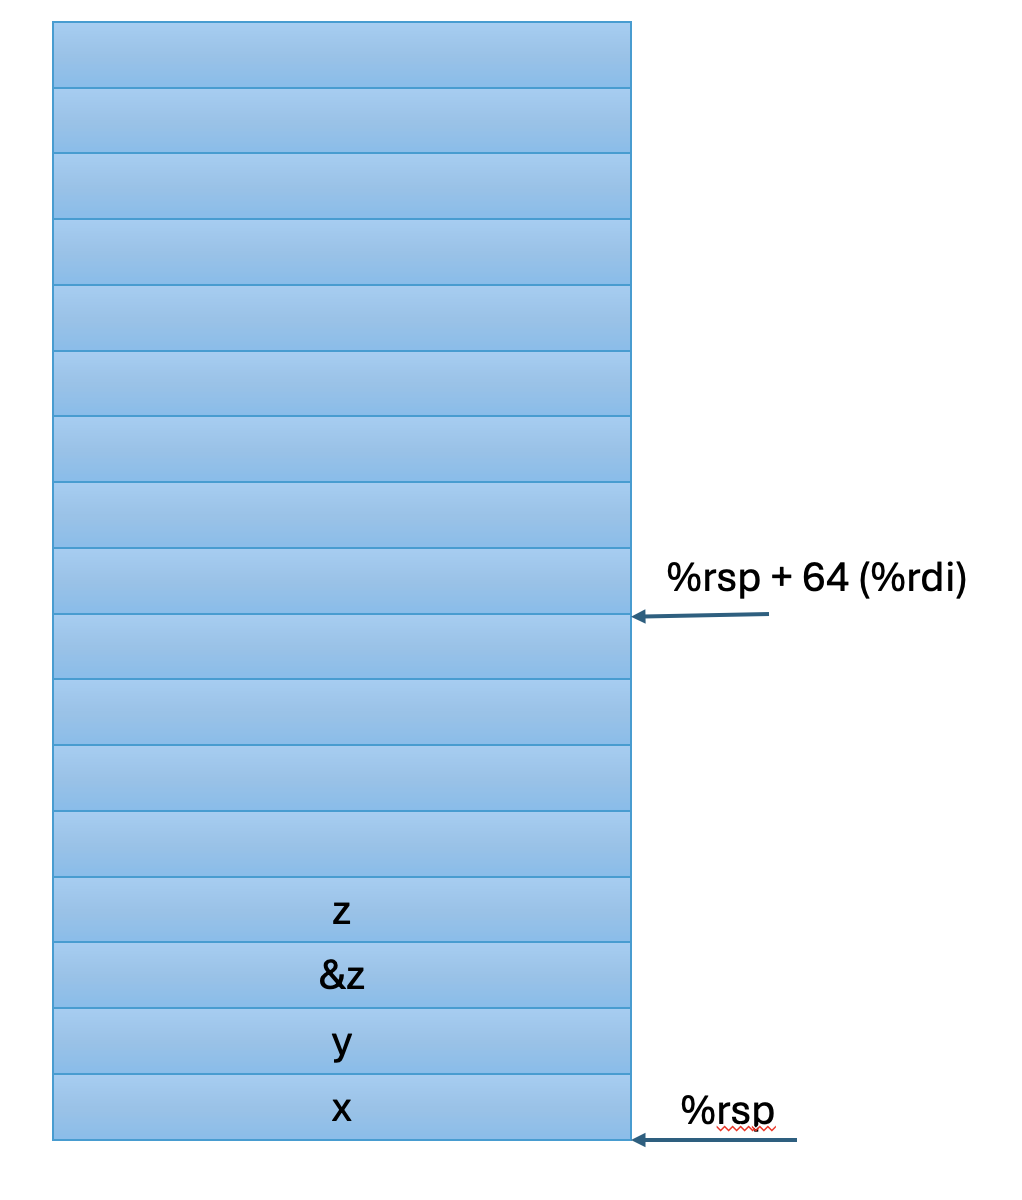
\includegraphics[width=0.5\textwidth]{stack1}
		\caption{Stack frame for eval}
		\label{fig:stack1}
	\end{figure}
	See figure \ref{fig:stack1}.
	\item \textbf{What value does eval pass in its call to process?} \\
	$\%rsp + 64$
	\item \textbf{How does the code for process access the elements of structure argument s?} \\
	by use \%rsp and offset.
	\item \textbf{How does the code for process set te fields of result structure r?} \\
	By use parameter passed from eval.
	\item \textbf{Complete your diagram of the stack frame for eval, showing how eval
	access the elements of structure r following the return from process.} \\
	\begin{figure}[h]
		\centering
		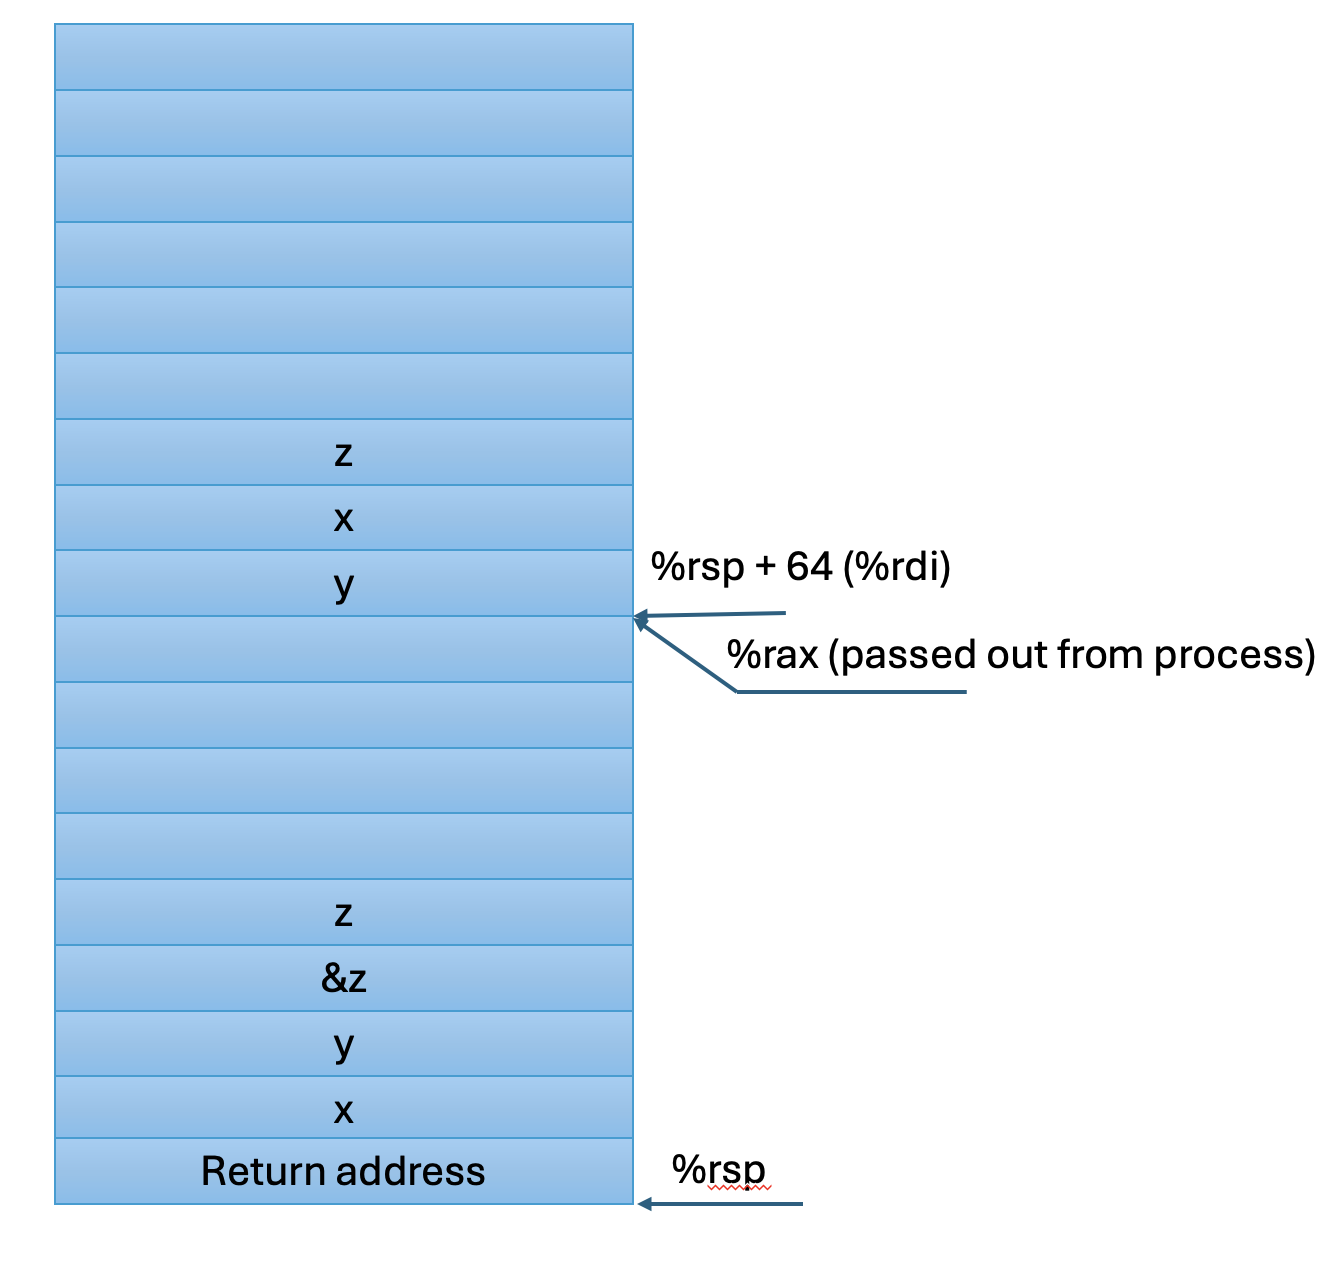
\includegraphics[width=0.5\textwidth]{stack2}
		\caption{Stack after call process}
		\label{fig:stack2}
	\end{figure}
	See figure \ref{fig:stack2}. The function eval access the elements of structure r
	by \%rsp and offset.
	\item \textbf{What general principles can you discern about how structure values
	are passed as function arguments and how they are returned as function results?} \\
	The space for the structure is allocated by the caller, and the address is passed
	as parameter. The result is accessed by caller using \%rsp and offset.
\end{enumerate}
\end{document}
